\documentclass[12pt]{article}
\usepackage[utf8]{inputenc}

%%% I added a few packages. This next one allows you to set the margins.
\usepackage[top=.5in,bottom=1in,right=.75in,left=.75in]{geometry}
\usepackage{multicol}
%\usepackage{newspaper}
\setlength{\columnsep}{1cm}
\usepackage{blindtext}
\usepackage{varwidth}

%%% This one does boxes in a really nice way.
\usepackage{tcolorbox}
\usepackage{mdframed}
\usepackage{minibox}
\usepackage{graphicx}
\graphicspath{ {./images/} }
\usepackage{epstopdf}
  \epstopdfDeclareGraphicsRule{.pdf}{png}{.png}{convert #1 \OutputFile}
  \DeclareGraphicsExtensions{.png,.pdf}
\usepackage{hyperref}
\hypersetup{
    colorlinks=true,
    linkcolor=blue,
    filecolor=magenta,      
    urlcolor=cyan,
    pdftitle={MSCSMess},
    pdfpagemode=FullScreen,
    }
\urlstyle{same}
 \usepackage{fix-cm}
 \usepackage{soul}
 \usepackage{graphicx}
 \usepackage{multicol}


\newcommand{\ds}{\displaystyle}
\newcommand{\ZZ}{\mathbb{Z}}
\newcommand{\QQ}{\mathbb{Q}}
\newcommand{\RR}{\mathbb{R}}
\newcommand{\CC}{\mathbb{C}}
\newcommand{\FF}{\mathbb{F}}
\newcommand{\xx}{\mathbf{x}}
\newcommand{\uu}{\mathbf{u}}
\newcommand{\vv}{\mathbf{v}}

\newcommand{\bolder}{\textbf}
 
 
\title{\fontsize{60}{70}\selectfont {\bf {MSCS} 
\includegraphics[scale=.3]{images/OleLion.png} {Mess}}}
\author{Department of Mathematics, Statistics, and Computer Science \\ St.\@ Olaf College, Northfield, MN 55057 \vspace{-2ex}} 
\date{\today\, $|$ Volume 54, No.\@ 15 \line(1,0){500}}


\begin{document}

\maketitle \vspace{-0.5cm}

Happy Friday, we hope everyone had a great week! Whether you are interested in research, exploring AI in education, or maybe even going into math education abroad... there is something here for everyone! Take a look at what we have going on below, and most importantly, have an amazing weekend!

 \begin{multicols}{2}

\begin{tcolorbox}[colback=white, colframe=black]
    \begin{center}
    \title{{\large \bolder{2/23 MSCS Colloquium}}}
    \end{center}
\end{tcolorbox}
Join us Monday, Feb 23 at 3:30 PM in RNS 210 for a talk by Alex Knutson, a statistical geneticist at Pfizer and St. Olaf alum. She will discuss how simple statistics and human genetics can guide drug discovery, introducing the HGSAR framework, which combines genetic data and lab measurements to identify new drug targets and understand disease traits. Alex will share examples of how this approach has validated existing drugs and uncovered novel targets. Don’t miss this chance to see how statistics and genetics advance medicine!

\begin{tcolorbox}[colback=white, colframe=black]
    \begin{center}
    \title{{\large \bolder{Computer Science Alumni Graduate School Panel}}}
    \end{center}
\end{tcolorbox}
Are you considering pursuing graduate school in computer science, data science, or electrical engineering? Come (virtually) to the Computer Science Alumni Graduate School Panel! This Monday, February 23rd at 6pm several Oles currently in graduate school will be discussing their experiences and answering questions. Panelists are pursuing both Masters degrees are Doctorates across the fields of computer science, computer engineering, electrical engineering, and data science. The panel will be held over Zoom. To join, use Meeting ID: 990 0082 6389 and passcode: 843176.

 \begin{tcolorbox}[colback=white, colframe=black]
    \begin{center}
    \title{{\large \bolder{Series on AI Literacy in Education}}}
    \end{center}
\end{tcolorbox}
Generative AI technology continues to make headlines and capture attention. As part of an independent study project this spring, this discussion series provides a platform for faculty and students to share ideas, ask questions, and explore the role of generative AI tools in the classroom. There will be three sessions during the first half of the semester. More information, including dates and session times, can be found on the poster below and at this \href{https://fortressokorie.github.io/ai_literacy/} {website}! The next session will take place on Thursday, March 5th, in RNS 356 from 11:30 AM to 12:30 PM. For any questions, please contact Fortress Okorie at okorie1@stolaf.edu.

\begin{tcolorbox}[colback=white, colframe=black]
    \begin{center}
    \title{{\large \bolder{Summer Opportunity in Math Education}}}
    \end{center}
\end{tcolorbox}

\href {https://bsmeducation.com} {Budapest Semesters in Mathematics Education (BSME)} is a 6-week summer program in Budapest, Hungary, designed for those interested in the learning and teaching of mathematics. Participants take a variety of courses in mathematics education and complete a week-long field experience. Come experience the \href{https://bsmeducation.com/wp-content/uploads/2020/02/hungarian-pedagogy-flyer.pdf}{Hungarian pedagogy} based on guided discovery—which emphasizes problem solving, mathematical creativity, and communication—as well as the rich and vibrant culture of Hungary.

Scholarships are available from the St. Olaf Financial Aid Office. See the \href{https://wp.stolaf.edu/smithcenter/st-olaf-summer-programs/#:~:text=All%20students%20are%20automatically%20considered%20for%20a%20need%2Dbased%20scholarship%20(see%20J%2DTerm%20column)%20of%20up%20to%2050%25%20of%20program%20costs%20from%20the%20St.%20Olaf%20Financial%20Aid%20Office.%C2%A0%C2%A0}{Smith Center's} webpage for more details. If you have any questions, contact Prof. Ryota Matsuura (matsuura@stolaf.edu).

\begin{tcolorbox}[colback=white, colframe=black]
    \begin{center}
    \title{{\large \bolder{Problem Solving Group}}}
    \end{center}
\end{tcolorbox}
The Math Problem Solving Group meets weekly to have fun, solve math problems, eat candy, and prepare for upcoming math contests. Meetings are Thursdays from 11:30 am - 12:30 pm, in RNS 207 (the Center for Interdisciplinary Research room). Everyone is welcome, regardless of prior experience in mathematics or math contests!


\end{multicols} \vspace{0.5cm}

\vfill

\begin{center}
    \includegraphics[height=0.95\textheight]{images/Colloquium Taylor Okonek.png}
\end{center}

\begin{center}
    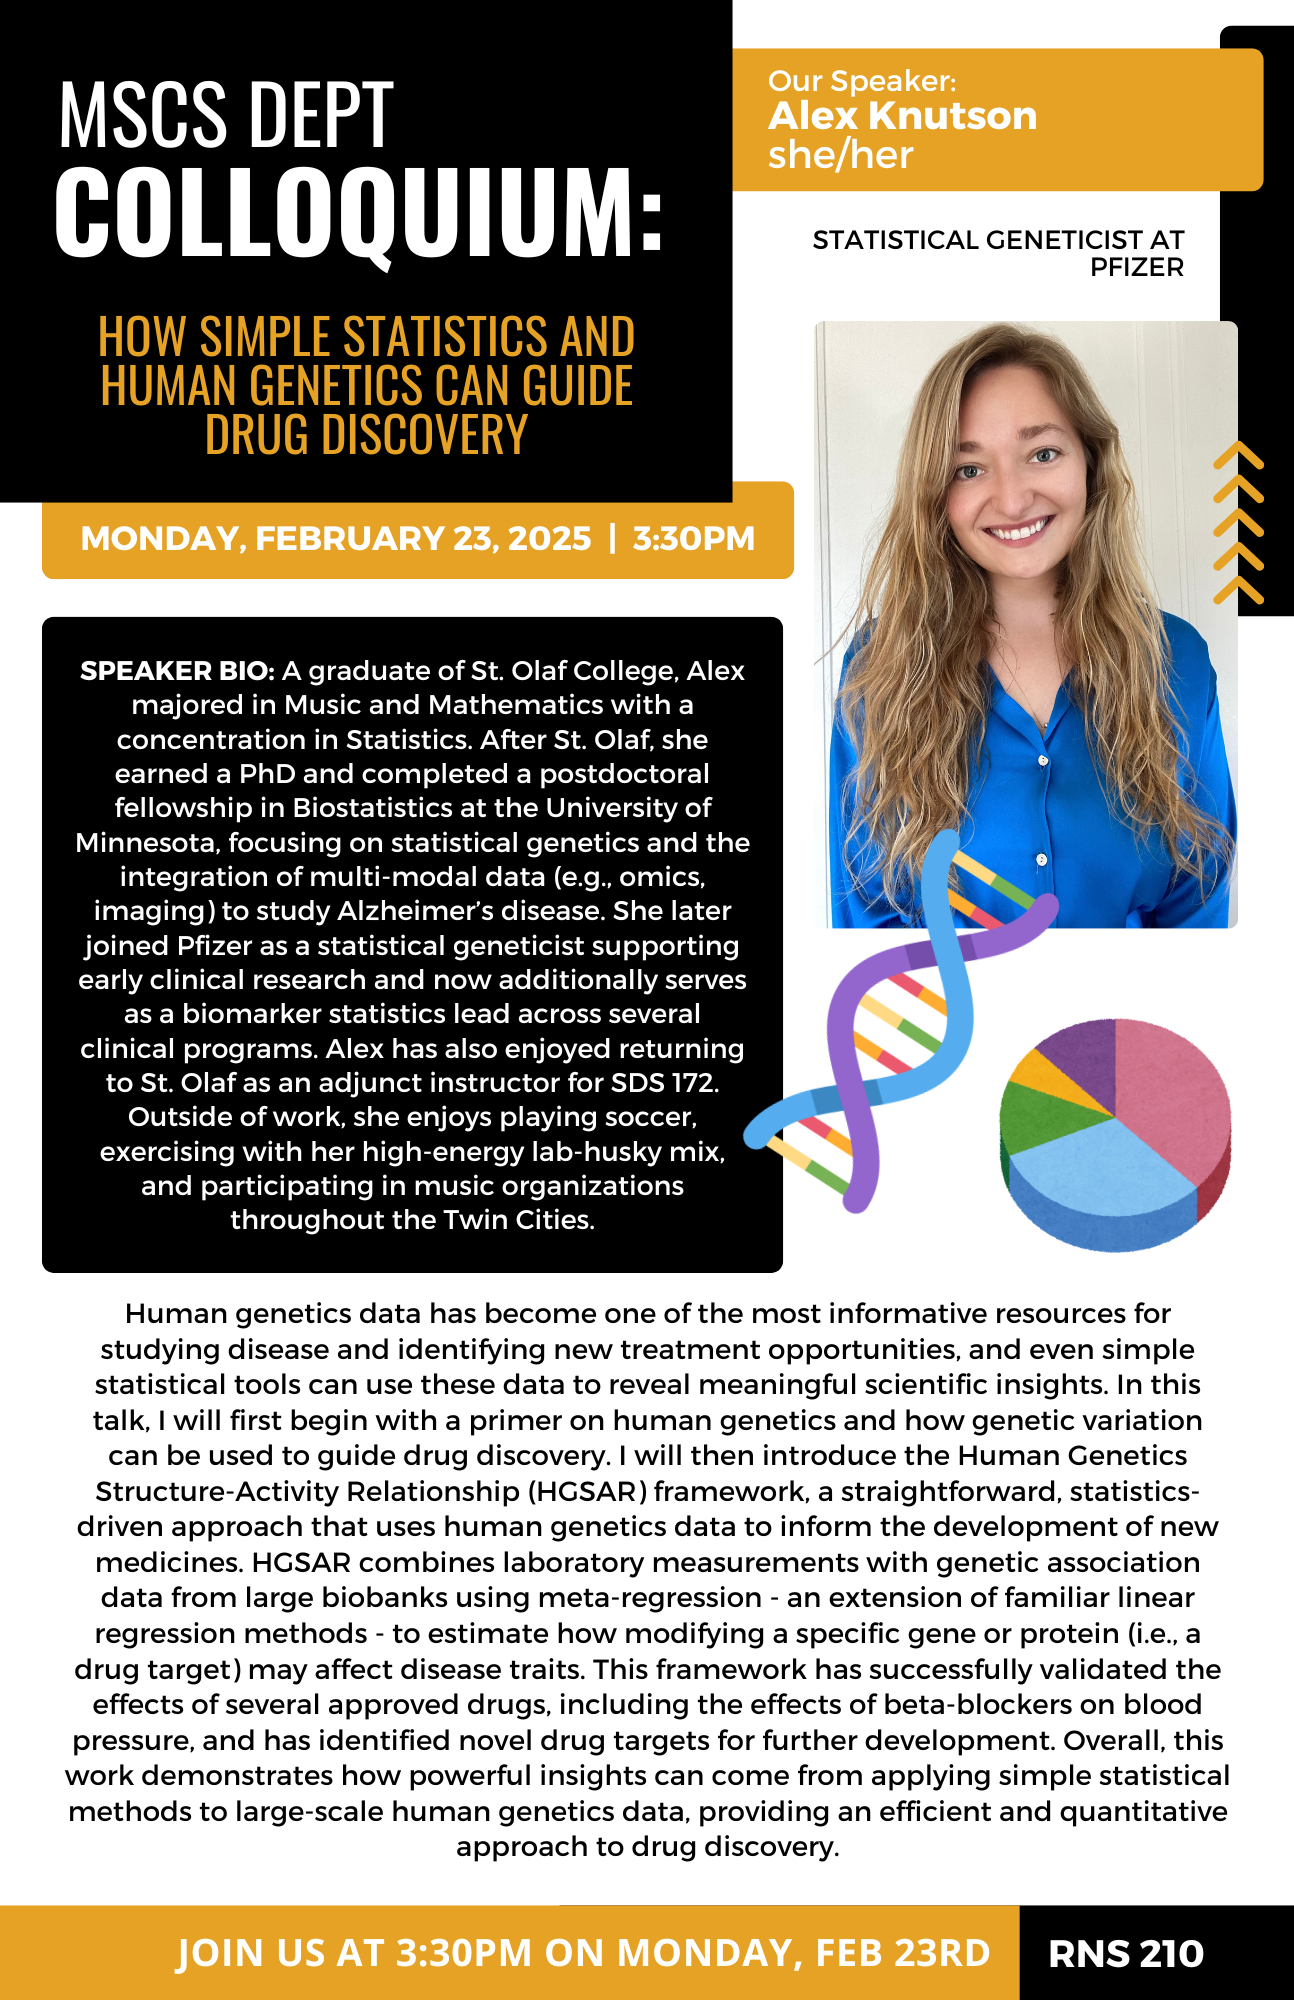
\includegraphics[height=0.95\textheight]{images/Colloquium Alex Knutson.png}
\end{center}

\begin{center}
    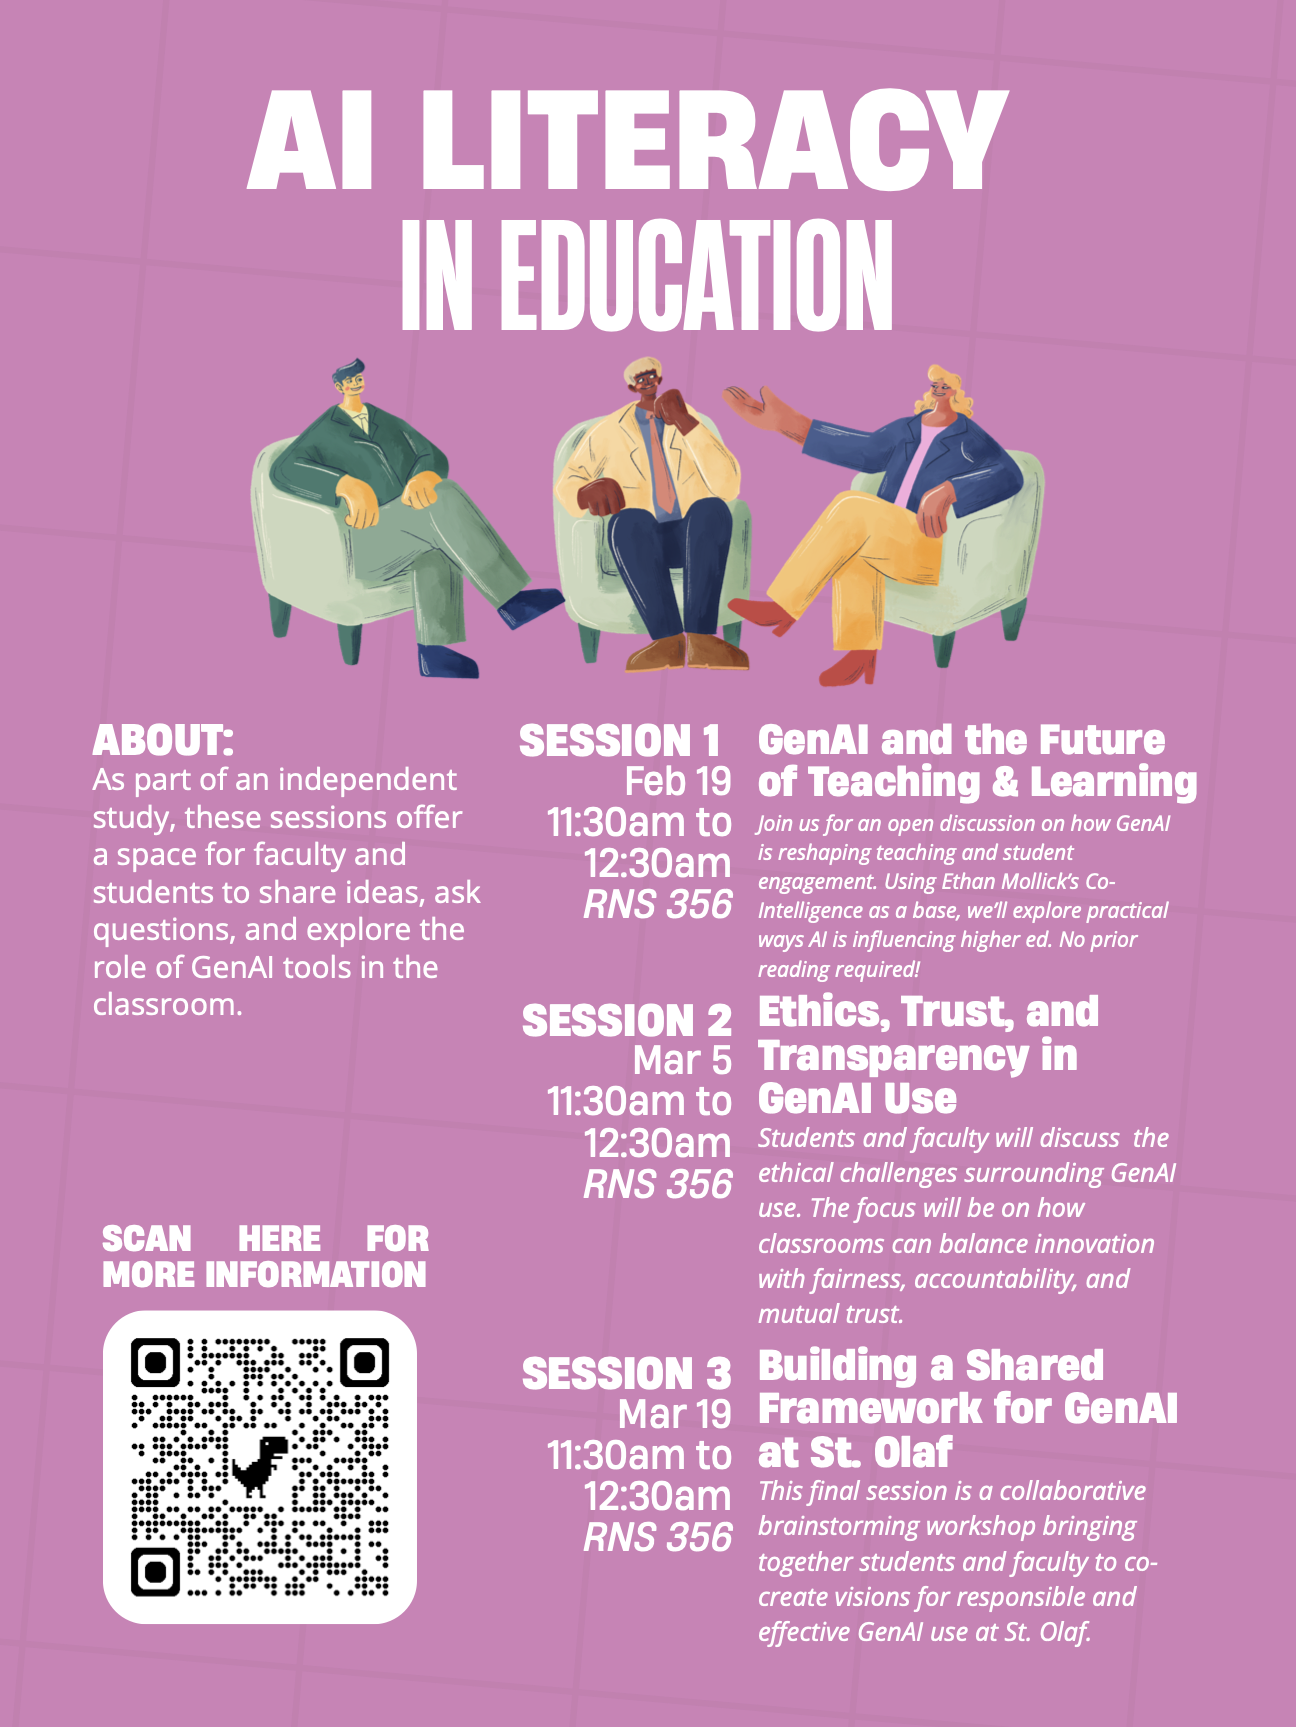
\includegraphics[height=0.95\textheight]{images/AI Literacy in Education2.png}
\end{center}

\begin{center}
    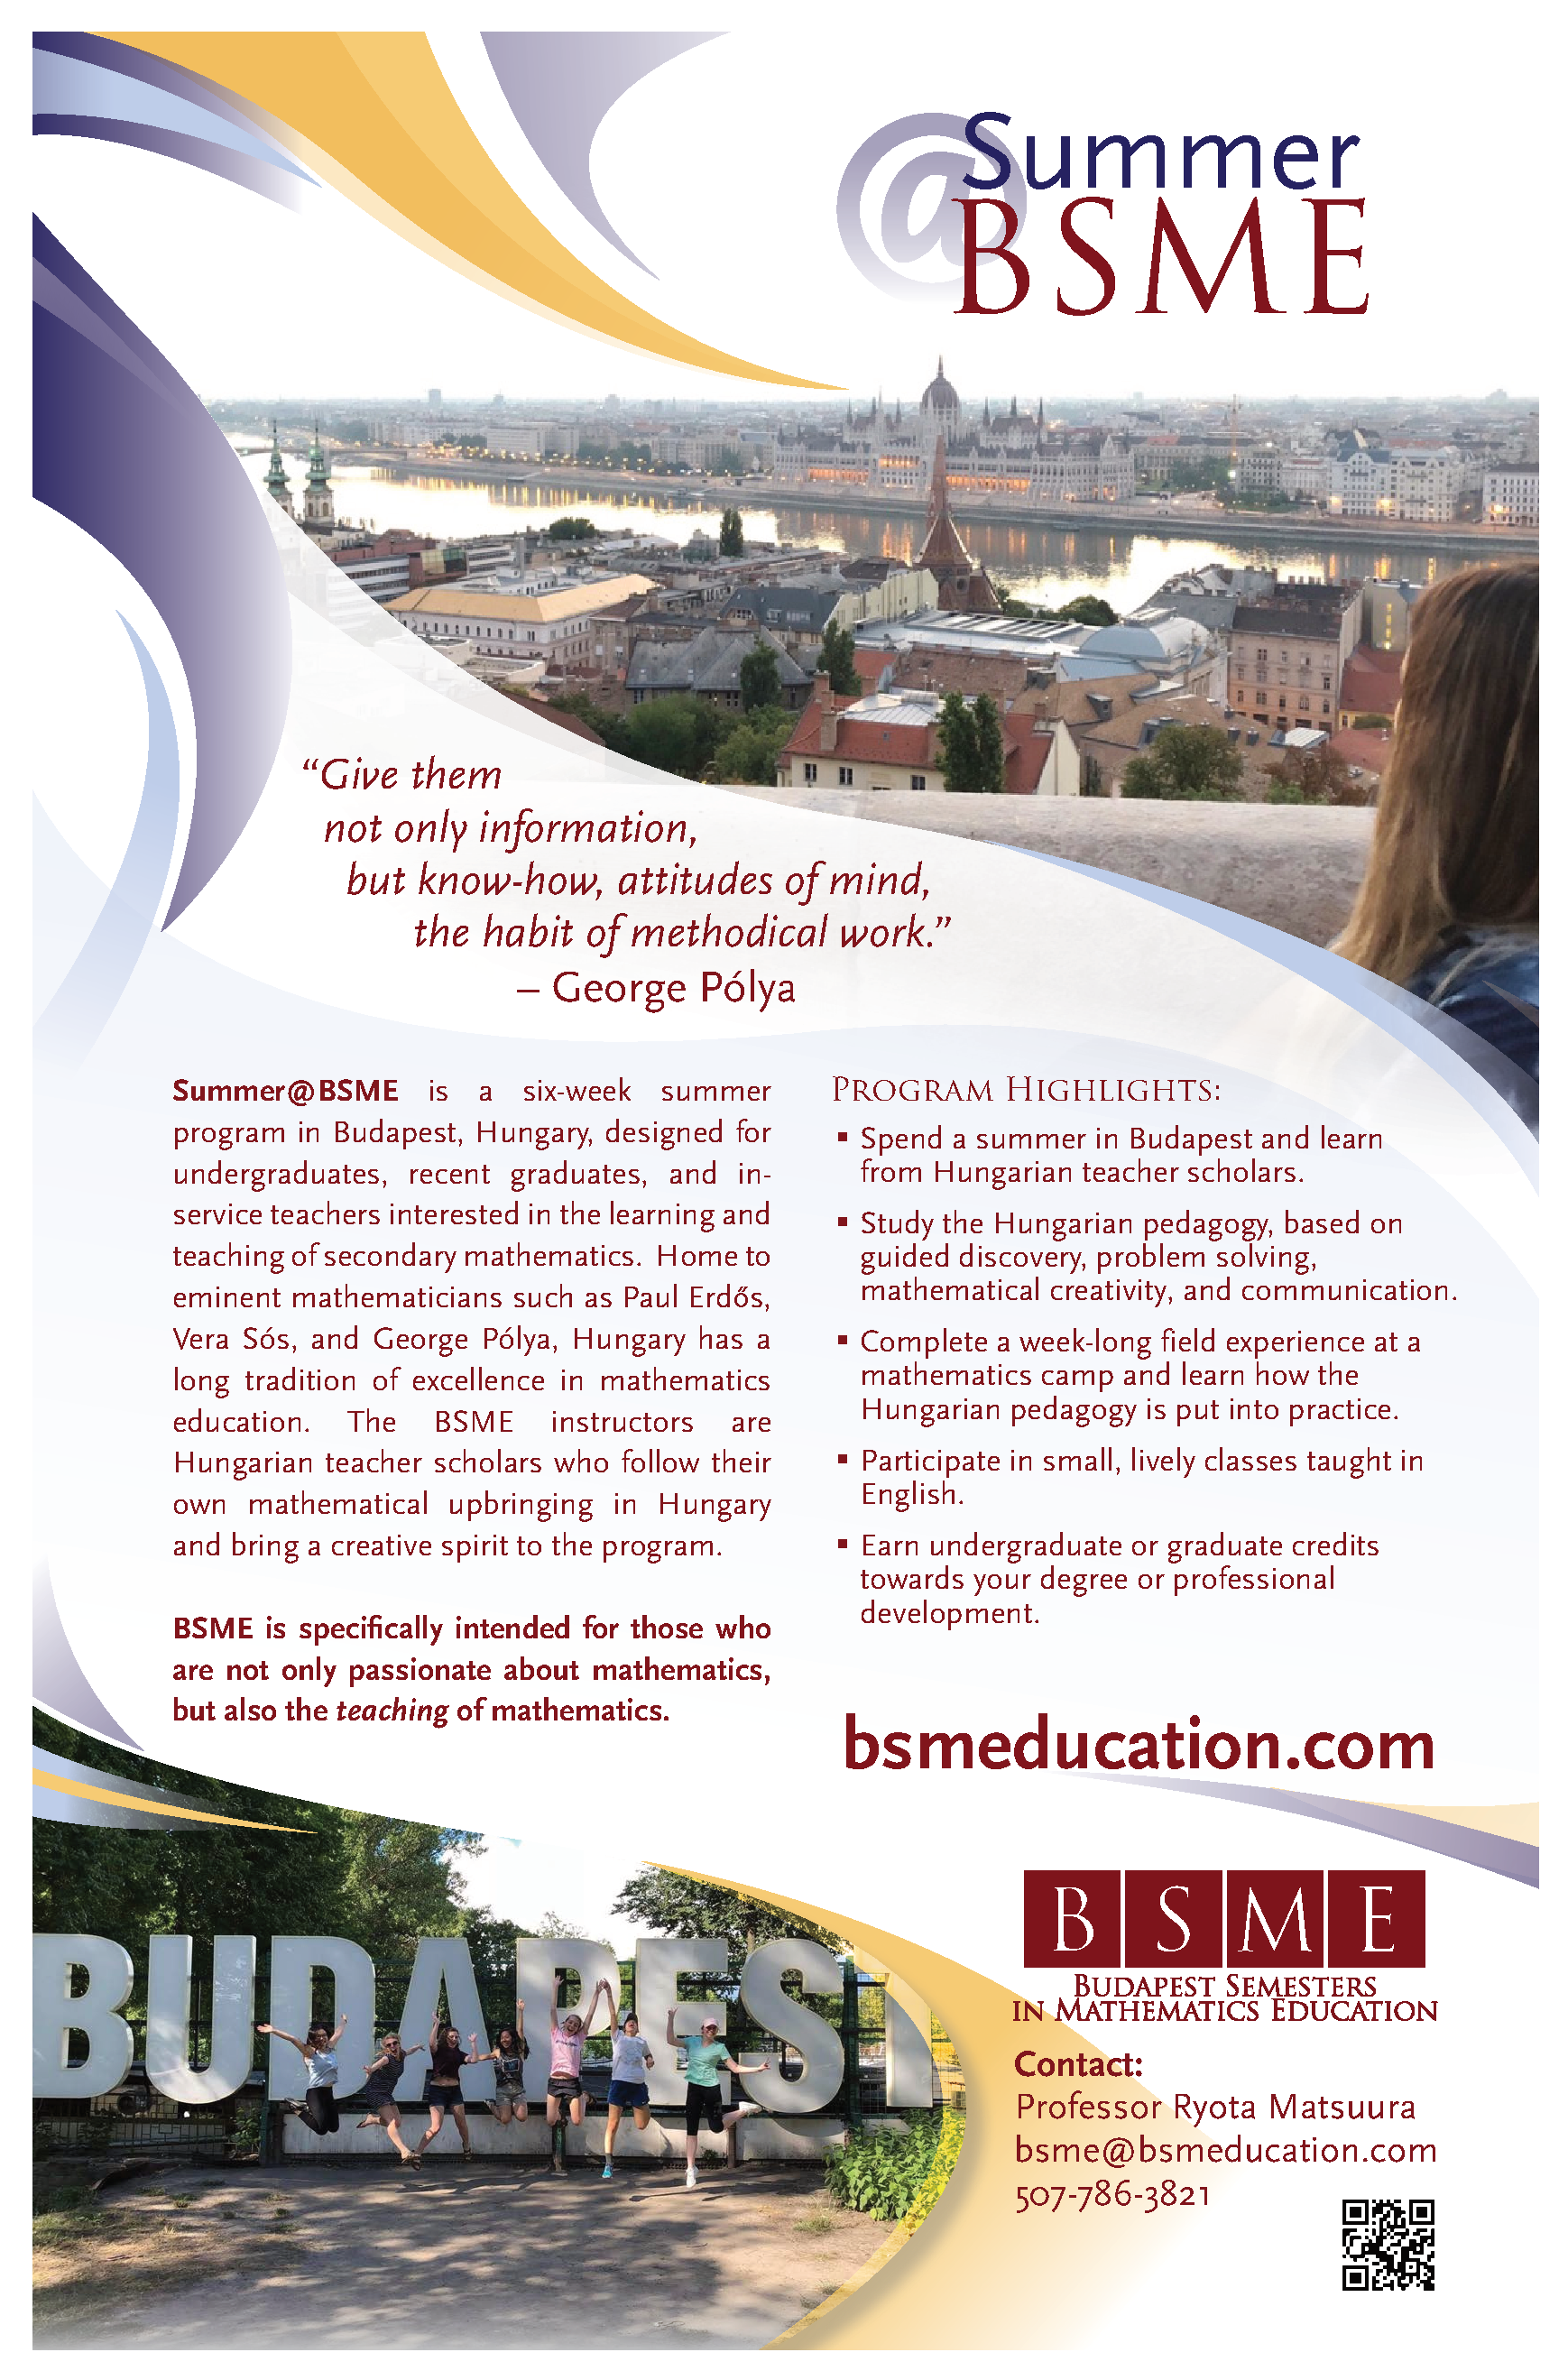
\includegraphics[height=0.95\textheight]{images/2024-bsme-poster-revised-web.pdf}
\end{center}

\begin{center}
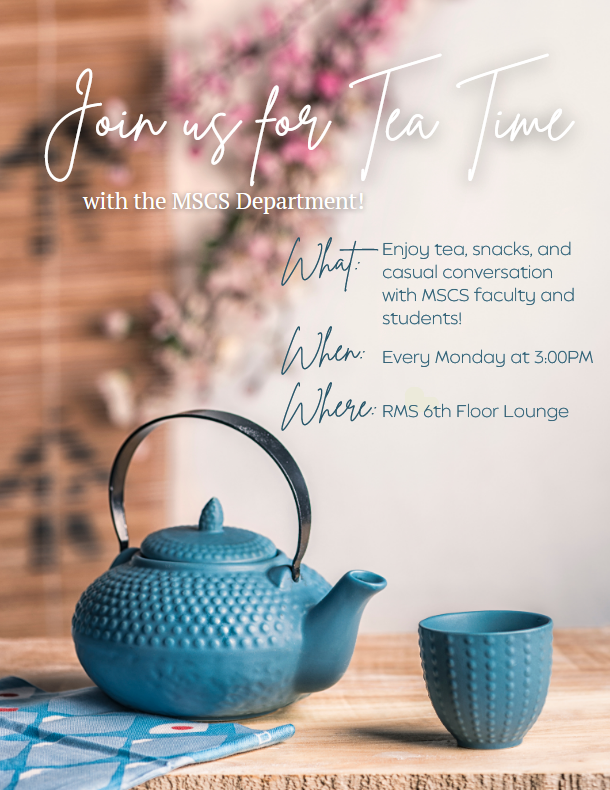
\includegraphics[width=0.9\textwidth]{images/Tea Time Poster.png}
\end{center}

\noindent{To submit an article, event, or anything else for publication in the Mess, email messeditor@stolaf.edu. Visit \href{https://wp.stolaf.edu/mscs/mscs-mess/}{http://wp.stolaf.edu/mscs/mscs-mess/} for a digital archive of previous MSCS Mess issues.}\\
	
\hfill Zach Martin \& Nima Dahir, Editors
	
\hfill Kyle Salois, Faculty Advisor


 

\end{document}